% -- Generated using the code: moving_clocks_resting_wrt_each_other_single_fig(0.3, 0, 6, 0.5)



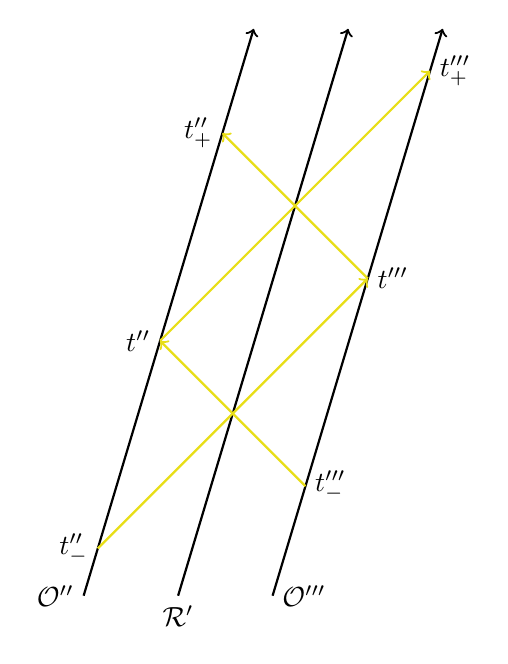
\begin{tikzpicture}[scale=1.2]
	% Draw lines of observers
	\draw[->, thick] (-1.0, 0) -- (0.7999999999999998, 6);
	\draw[->, thick] (1.0, 0) -- (2.8, 6);
	\draw[->, thick] (0.0, 0) -- (1.7999999999999998, 6);
	
	% Draw trajectories of light
	\draw[->, thick, black!10!yellow] (-0.85, 0.5) -- (2.007142857142857, 3.357142857142857);
	\draw[->, thick, black!10!yellow] (2.007142857142857, 3.357142857142857) -- (0.4686813186813188, 4.895604395604396);
	\draw[->, thick, black!10!yellow] (1.347802197802198, 1.1593406593406594) -- (-0.19065934065934043, 2.697802197802198);
	\draw[->, thick, black!10!yellow] (-0.19065934065934065, 2.697802197802198) -- (2.666483516483517, 5.554945054945055);
	
	% Make labels
	\draw (-1.0, 0) node[left] {$\mathcal{O}''$};
	\draw (-0.85, 0.5) node[left] {$t''_-$};
	\draw (0.4686813186813188, 4.895604395604396) node[left] {$t''_+$};
	\draw (2.007142857142857, 3.357142857142857) node[right] {$t'''$};
	\draw (1.0, 0) node[right] {$\mathcal{O}'''$};
	\draw (1.347802197802198, 1.1593406593406594) node[right] {$t'''_-$};
	\draw (2.6664835164835163, 5.554945054945055) node[right] {$t'''_+$};
	\draw (-0.19065934065934065, 2.697802197802198) node[left] {$t''$};
	\draw (0.0, 0) node[below] {$\mathcal{R}'$};
\end{tikzpicture}